\documentclass[10pt]{article}
\usepackage[a4paper,margin=18mm]{geometry}
\usepackage{amsmath,amssymb,booktabs,array,enumitem,longtable}
\usepackage[T1]{fontenc}\usepackage{lmodern}
\usepackage{tikz}\usetikzlibrary{shapes.gates.logic.US,positioning,arrows.meta,patterns,calc}
\usepackage[hidelinks]{hyperref}
\setlength{\parindent}{0pt}\setlength{\parskip}{4pt}\setlength{\emergencystretch}{2em}
\newcommand{\VDD}{V_{DD}}
\newcommand{\mos}[4]{\begin{scope}[shift={(#1,#2)}]
\draw (0,.24)--(0,-.24);\draw (0,.20)--(.25,.20)--(.25,.5);
\draw (0,-.20)--(.25,-.20)--(.25,-.5);\draw (-.16,.23)--(-.16,-.23);
\ifnum#4=1\draw (-.26,0) circle (.06);\draw (-.75,0)--(-.32,0);\else\draw (-.75,0)--(-.16,0);\fi
\node[anchor=east,font=\scriptsize] at (-.76,0) {$#3$};\end{scope}}
\newcommand{\ground}[2]{\draw (#1,#2)--(#1,{#2-.12});\draw ({#1-.17},{#2-.12})--({#1+.17},{#2-.12});\draw ({#1-.11},{#2-.20})--({#1+.11},{#2-.20});}
\newcommand{\rail}[3]{\draw (#1,#2)--(#1,{#2+.14});\node[above,font=\scriptsize] at (#1,{#2+.14}) {$#3$};}
\newcommand{\hmos}[4]{\begin{scope}[shift={(#1,#2)}]
\draw(-.24,0)--(.24,0);\draw(-.2,0)--(-.2,-.25)--(-.5,-.25);\draw(.2,0)--(.2,-.25)--(.5,-.25);
\draw(-.23,.16)--(.23,.16);
\ifnum#4=1\draw(0,.26)circle(.06);\draw(0,.32)--(0,.75);\else\draw(0,.16)--(0,.75);\fi
\node[below,font=\scriptsize]at(0,-.32){#3};\end{scope}}
\newcommand{\qheading}[1]{\par\medskip\textbf{#1}\par}
\begin{document}
\begin{center}{\Large\bfseries 2012 Archive Midterm---Independent Solutions}\\EE3032 Introduction to VLSI\end{center}
All seven questions are available. The six photographed question panels do not expose a printed year: 2012 is the archive attribution. The matching six student-answer photos also occur byte-for-byte under 2013, so that directory label is not independent dating evidence. They match this paper's functions, transistor labels and numerical premises, and are treated as fallible references. Student identity remains local.
Ideal switch-graph proofs and analytical RC/region/slack checks are reproducible in \texttt{verify\_logic\_timing.py}. No process simulation or measured transistor timing/power is claimed.
\qheading{1. Brief concepts (30 points)}
\begin{enumerate}[label=(\alph*),leftmargin=7mm]
\item CMP planarizes accumulated surface topography so later layers can be patterned and connected reliably. Uneven steps otherwise complicate lithography and fine-line continuity.
\item Pattern density affects polishing and etch uniformity. Local minimum/maximum density constraints, with fill where necessary, help control dishing/erosion and material thickness rather than leaving sparse/dense regions to process differently.
\item During plasma processing, a large floating conductor attached to a small MOS gate can collect charge. The resulting gate-oxide stress can damage the oxide. Antenna rules limit the relevant conductor/gate ratio or provide discharge paths; this is a fabrication charging effect, not normal radio reception. These first three points follow Li's \href{https://www.ee.ncu.edu.tw/jfli/public_html/VLSI/lecture/ch03.pdf}{fabrication lecture}, slides 8, 37--40.
\item The pMOS source is at $V_{DD}$, the nMOS source at $V_{SS}$, and both drains join the output. Both gates join the input. The following drawing labels those terminals explicitly.
\item $NM_L=V_{IL}-V_{OL}$ and $NM_H=V_{OH}-V_{IH}$. $V_{IL}$ and $V_{IH}$ are the two transfer-curve points with slope $-1$; $V_{OL}$ and $V_{OH}$ are the corresponding guaranteed output limits.
\item Increase separation/reduce parallel run length, and insert a grounded/power shield between the wires. These reduce mutual coupling. Buffering may improve victim drive and reduce coupled segment length but its effect depends on the aggressor/victim timing.
\item Fanout input-gate capacitance, output diffusion/junction capacitance, and wire capacitance (including relevant coupling).
\item At $V_{in}=V_{out}=V_{DD}/2$, equate the n/p currents. In the long-channel saturation approximation,
\[\mu_n(W/L)_n\left(V_{DD}/2-V_{tn}\right)^2
=\mu_p(W/L)_p\left(V_{DD}/2-|V_{tp}|\right)^2.\]
If threshold magnitudes match, $(W/L)_p=(\mu_n/\mu_p)(W/L)_n$. Equal geometric widths alone do not generally center the switching point; no mobility ratio is supplied in Q1.
\item Double-gate FinFET (control on the two fin sidewalls) and tri-gate FinFET (sidewalls plus the fin top). The double-gate structure is documented in \href{https://www2.eecs.berkeley.edu/Colloquium/Archives/11-12/Fall2011/kingliu-presentation.pdf}{Tsu-Jae King Liu's 2011 Berkeley lecture}, slide 19; Intel's \href{https://www.intc.com/news-events/press-releases/detail/655/intel-reinvents-transistors-using-new-3-d-structure}{2011 Tri-Gate announcement} describes three-side control. These are geometries, not an assertion that source/drain are extra gates.
\item Insert repeaters and split the wire into $N$ shorter driven segments. Its ideal wire contribution becomes $N k(\ell/N)^2=k\ell^2/N$, but the repeaters add approximately $Nt_b$. The optimum of that simple model is $N\simeq\ell\sqrt{k/t_b}$, giving roughly linear length scaling. Use noninverting buffers or preserve inverter parity. Without repeater delay data there is no numerical optimum count.
\end{enumerate}
\begin{center}\begin{tikzpicture}[x=.8cm,y=.8cm,font=\scriptsize]
\draw[->](0,0)--(5,0)node[right]{$V_{in}$};\draw[->](0,0)--(0,4)node[above]{$V_{out}$};
\draw plot[smooth]coordinates{(0,3.5)(1,3.4)(1.6,3.1)(2.1,2.6)(2.5,1.7)(2.9,.8)(3.4,.35)(4.5,.25)};
\draw[dashed](0,3.1)--(1.6,3.1)--(1.6,0);\draw[dashed](0,.8)--(2.9,.8)--(2.9,0);\node[left]at(0,3.1){$V_{OH}$};\node[left]at(0,.8){$V_{OL}$};\node[below]at(1.6,0){$V_{IL}$};\node[below]at(2.9,0){$V_{IH}$};
\end{tikzpicture}\quad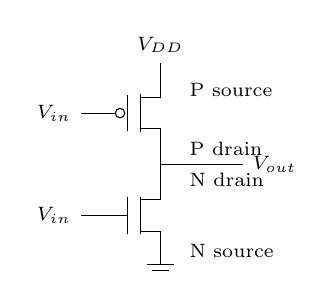
\begin{tikzpicture}[x=1cm,y=1cm,font=\scriptsize]
\mos{0}{1.5}{V_{in}}{1}\mos{0}{.2}{V_{in}}{0}\draw(.25,1)--(.25,.7);\draw(.25,.85)--(1.3,.85)node[right]{$V_{out}$};\rail{.25}{2}{V_{DD}}\ground{.25}{-.3}
\node[right]at(.5,1.8){P source};\node[right]at(.5,1.05){P drain};\node[right]at(.5,.65){N drain};\node[right]at(.5,-.25){N source};
\end{tikzpicture}\end{center}
\textbf{Student comparison.} Noise-margin and centering equations are consistent when equal threshold magnitudes are stated. The student's unqualified two-times pMOS width is not justified for Q1's unspecified mobility ratio. Its crosstalk buffering/twisting suggestions are possible engineering choices, but increased spacing/shielding directly addresses mutual coupling without added-delay assumptions.
\qheading{2. Complete majority-gate Elmore model (15 points)}
\begin{center}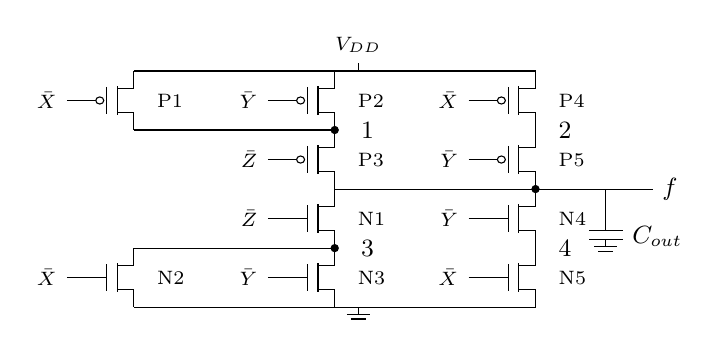
\begin{tikzpicture}[x=.85cm,y=.75cm,font=\small]
\mos{0}{6}{\bar X}{1}\mos{3}{6}{\bar Y}{1}\mos{3}{5}{\bar Z}{1}\mos{6}{6}{\bar X}{1}\mos{6}{5}{\bar Y}{1}
\draw(.25,6.5)--(6.25,6.5);\rail{3.6}{6.5}{V_{DD}}\draw(.25,5.5)--(3.25,5.5);\fill(3.25,5.5)circle(1.5pt);\node[right]at(3.5,5.5){1};\node[right]at(6.45,5.5){2};
\draw(3.25,4.5)--(8.0,4.5)node[right]{$f$};\fill(6.25,4.5)circle(1.5pt);
\mos{3}{4}{\bar Z}{0}\mos{0}{3}{\bar X}{0}\mos{3}{3}{\bar Y}{0}\mos{6}{4}{\bar Y}{0}\mos{6}{3}{\bar X}{0}
\draw(.25,3.5)--(3.25,3.5);\fill(3.25,3.5)circle(1.5pt);\node[right]at(3.5,3.5){3};\node[right]at(6.45,3.5){4};
\draw(.25,2.5)--(6.25,2.5);\ground{3.6}{2.5}
\foreach\x/\y/\n in {0/6/P1,3/6/P2,3/5/P3,6/6/P4,6/5/P5,3/4/N1,0/3/N2,3/3/N3,6/4/N4,6/3/N5}{\node[right,font=\scriptsize]at(\x+.45,\y){\n};}
\draw(7.3,4.5)--(7.3,3.8);\draw(7.05,3.8)--(7.55,3.8);\draw(7.05,3.65)--(7.55,3.65);\ground{7.3}{3.65}\node[right]at(7.55,3.7){$C_{out}$};
\end{tikzpicture}\\\small Figure 1: Transistor-level schematic.\end{center}
The p-network conducts for $Z(X+Y)+XY$; the n-network conducts for $\bar Z(\bar X+\bar Y)+\bar X\bar Y$. Thus
\[\boxed{f=XY+XZ+YZ},\]
with complementary exclusive rail paths for all eight input combinations. The supplied allowed set is only six of those combinations.
\textbf{(a) Worst Elmore first moments:}
\[\boxed{\tau_{r,max}=R_p(3C+2C_{out}),\qquad \tau_{f,max}=R_n(3C+2C_{out}).}\]
For a rise ending at 110, P4 and P5 form the two-resistor main path. Node 2 contributes $R_pC_2$. N1 remains ON because $\bar Z=1$, attaching node 3 to the output even though N2/N3 are OFF. Its capacitance contributes $2R_pC_3$, along with $2R_pC_{out}$:
\[\tau_r=R_pC_2+2R_p(C_3+C_{out})=R_p(3C+2C_{out}).\]
For a fall ending at 010, N1 and N2 form the main path. Node 3 contributes $R_nC_3$; P5 remains ON and attaches node 2 despite P4 being OFF:
\[\tau_f=R_nC_3+2R_n(C_2+C_{out})=R_n(3C+2C_{out}).\]
These are attained in the stated constant-on-resistance, full-level RC step model by the allowed single-input $010\leftrightarrow110$ transition: all three participating capacitors start with the full opposite-level error. Other prior states may precharge an internal node and reduce its contribution. Real threshold-limited internal swings would require an initial-voltage/current model not supplied in part (a). OFF devices disconnect branches; they do not disconnect a capacitor if a different ON device still joins it to the output.
\newpage
The complete final ON-network first moments, normalized to the appropriate rail resistance, are:
\begin{center}\begin{tabular}{clll}\toprule Final $XYZ$&$f$&Edge&Normalized first moment\\\midrule
000&0&fall&$(5C+6C_{out})/7$\\
010&0&fall&$3C+2C_{out}$\\
100&0&fall&$3C+2C_{out}$\\
110&1&rise&$3C+2C_{out}$\\
101&1&rise&$3C+2C_{out}$\\
111&1&rise&$(5C+6C_{out})/7$\\\bottomrule\end{tabular}\end{center}
For 000/111, the two conducting branches have resistances $3R/2$ and $2R$ in parallel; the effective output resistance is $6R/7$. The two main internal capacitor weights are $2R/7$ and $3R/7$. The verifier solves the complete resistor conductance matrix with exact rational arithmetic, including dangling attached branches. It separately varies $R_n,R_p$ to check that the reported coefficients do not depend on the opposite-network branch resistance.
Elmore is a \emph{first moment}, not an exact multi-pole 10--90\% rise/fall interval. If the course uses the customary one-pole edge estimate, report $t_{10-90}\simeq\ln9\,\tau\simeq2.2\tau$ with that convention explicitly stated. No unique measured edge in seconds can be inferred without $R,C,C_{out}$ values and input slew.
The student's full-credit expression $R(C+2C_{out})$ accounts only for the main branch. It omits node 3 during the worst rise and node 2 during the worst fall, so it is not adopted for the printed full capacitance graph.
\textbf{(b) Internal switching power.} Define $\alpha_i$ as the expected number/probability of charging events per clock cycle (0$\to$1 activity). A partial-swing capacitor charged from the supply draws charge $C_iV_i$, so
\[\boxed{P_{int}=fV_{DD}\sum_{i=1}^{4}\alpha_i C_iV_i
=fCV_{DD}(\alpha_1V_1+\alpha_2V_2+\alpha_3V_3+\alpha_4V_4).}\]
If ``activity'' instead counts both rising and falling transitions symmetrically, replace each $\alpha_i$ above by $\alpha_i/2$. The output load is excluded because the question asks \emph{internal} cell power. Leakage and short-circuit currents require separate data. The matching student's supply-times-swing expression is consistent with the charging-event convention.
\newpage
\qheading{3. Dual-$V_t$ transistor allocation (10 points)}
The exact network is NAND2$\to$NOR2$\to$OR2 on $O_0$, and NOR2/INV$\to$NAND2 on $O_1$. A static CMOS OR2 is a NOR2 plus an inverter. Define the intermediate nodes
\[a=\overline{I_1I_2},\quad b=\overline{I_0+a},\quad c=\overline{b+I_3},\quad e=\overline{I_3+I_4},\quad v=\bar I_5.\]
Then $O_0=\bar c=\bar I_0I_1I_2+I_3$ and $O_1=\overline{ev}=I_3+I_4+I_5$. The circuit has 24 MOS, not one device per logic symbol.
\textbf{Conditional transistor schematic.} The following allocation uses thin/high-$V_t$ devices in the entire ten-device $O_1$ cone and in two shorter parallel nMOS branches ($BN1$ gated by $I_0$, and $CN2$ gated by $I_3$). The other 12 devices on the critical serial paths remain thick/low-$V_t$. H/L is also printed next to every name for legibility.
\begin{center}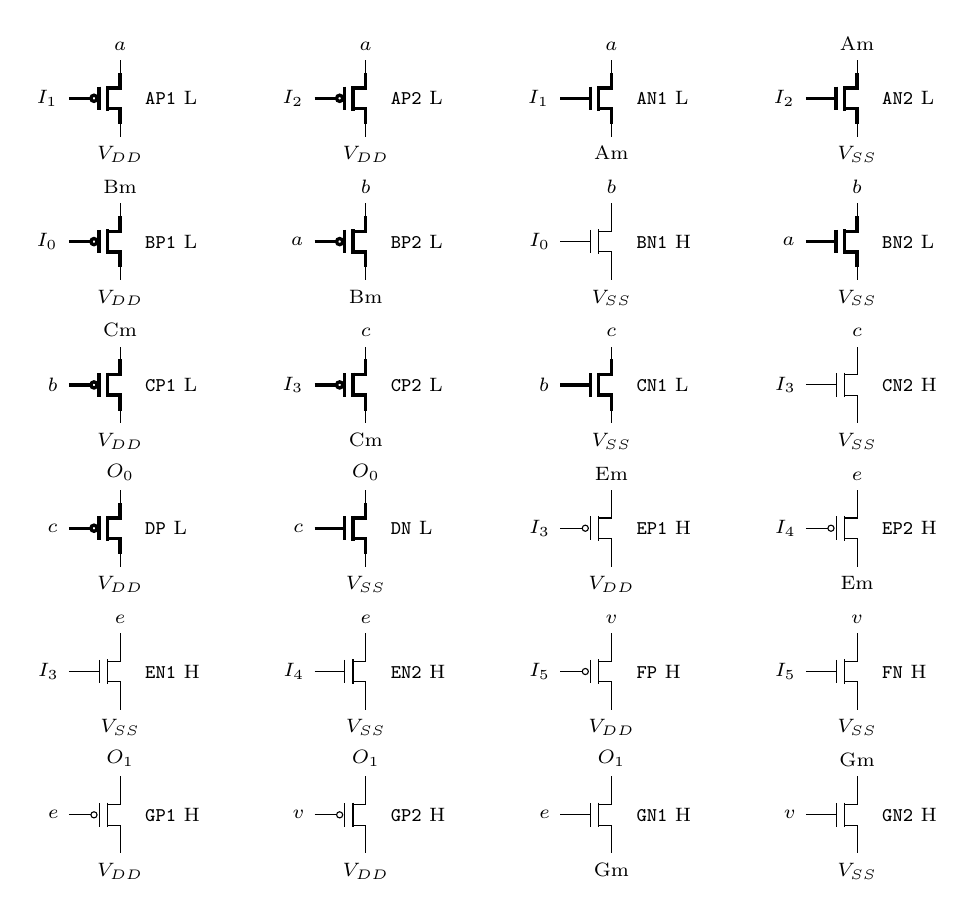
\begin{tikzpicture}[x=0.65cm,y=0.65cm,font=\scriptsize]
\begin{scope}[very thick]\mos{0.0}{0.0}{I_1}{1}\end{scope}
\draw(0.25,0.5)--(0.25,0.75)node[above]{$ a $};
\draw(0.25,-0.5)--(0.25,-0.75)node[below]{$ V_{DD} $};
\node[anchor=west]at(0.55,0.0){\texttt{AP1} L};
\begin{scope}[very thick]\mos{4.8}{0.0}{I_2}{1}\end{scope}
\draw(5.05,0.5)--(5.05,0.75)node[above]{$ a $};
\draw(5.05,-0.5)--(5.05,-0.75)node[below]{$ V_{DD} $};
\node[anchor=west]at(5.35,0.0){\texttt{AP2} L};
\begin{scope}[very thick]\mos{9.6}{0.0}{I_1}{0}\end{scope}
\draw(9.85,0.5)--(9.85,0.75)node[above]{$ a $};
\draw(9.85,-0.5)--(9.85,-0.75)node[below]{$ \mathrm{Am} $};
\node[anchor=west]at(10.15,0.0){\texttt{AN1} L};
\begin{scope}[very thick]\mos{14.399999999999999}{0.0}{I_2}{0}\end{scope}
\draw(14.649999999999999,0.5)--(14.649999999999999,0.75)node[above]{$ \mathrm{Am} $};
\draw(14.649999999999999,-0.5)--(14.649999999999999,-0.75)node[below]{$ V_{SS} $};
\node[anchor=west]at(14.95,0.0){\texttt{AN2} L};
\begin{scope}[very thick]\mos{0.0}{-2.8}{I_0}{1}\end{scope}
\draw(0.25,-2.3)--(0.25,-2.05)node[above]{$ \mathrm{Bm} $};
\draw(0.25,-3.3)--(0.25,-3.55)node[below]{$ V_{DD} $};
\node[anchor=west]at(0.55,-2.8){\texttt{BP1} L};
\begin{scope}[very thick]\mos{4.8}{-2.8}{a}{1}\end{scope}
\draw(5.05,-2.3)--(5.05,-2.05)node[above]{$ b $};
\draw(5.05,-3.3)--(5.05,-3.55)node[below]{$ \mathrm{Bm} $};
\node[anchor=west]at(5.35,-2.8){\texttt{BP2} L};
\begin{scope}[thin]\mos{9.6}{-2.8}{I_0}{0}\end{scope}
\draw(9.85,-2.3)--(9.85,-2.05)node[above]{$ b $};
\draw(9.85,-3.3)--(9.85,-3.55)node[below]{$ V_{SS} $};
\node[anchor=west]at(10.15,-2.8){\texttt{BN1} H};
\begin{scope}[very thick]\mos{14.399999999999999}{-2.8}{a}{0}\end{scope}
\draw(14.649999999999999,-2.3)--(14.649999999999999,-2.05)node[above]{$ b $};
\draw(14.649999999999999,-3.3)--(14.649999999999999,-3.55)node[below]{$ V_{SS} $};
\node[anchor=west]at(14.95,-2.8){\texttt{BN2} L};
\begin{scope}[very thick]\mos{0.0}{-5.6}{b}{1}\end{scope}
\draw(0.25,-5.1)--(0.25,-4.85)node[above]{$ \mathrm{Cm} $};
\draw(0.25,-6.1)--(0.25,-6.35)node[below]{$ V_{DD} $};
\node[anchor=west]at(0.55,-5.6){\texttt{CP1} L};
\begin{scope}[very thick]\mos{4.8}{-5.6}{I_3}{1}\end{scope}
\draw(5.05,-5.1)--(5.05,-4.85)node[above]{$ c $};
\draw(5.05,-6.1)--(5.05,-6.35)node[below]{$ \mathrm{Cm} $};
\node[anchor=west]at(5.35,-5.6){\texttt{CP2} L};
\begin{scope}[very thick]\mos{9.6}{-5.6}{b}{0}\end{scope}
\draw(9.85,-5.1)--(9.85,-4.85)node[above]{$ c $};
\draw(9.85,-6.1)--(9.85,-6.35)node[below]{$ V_{SS} $};
\node[anchor=west]at(10.15,-5.6){\texttt{CN1} L};
\begin{scope}[thin]\mos{14.399999999999999}{-5.6}{I_3}{0}\end{scope}
\draw(14.649999999999999,-5.1)--(14.649999999999999,-4.85)node[above]{$ c $};
\draw(14.649999999999999,-6.1)--(14.649999999999999,-6.35)node[below]{$ V_{SS} $};
\node[anchor=west]at(14.95,-5.6){\texttt{CN2} H};
\begin{scope}[very thick]\mos{0.0}{-8.399999999999999}{c}{1}\end{scope}
\draw(0.25,-7.899999999999999)--(0.25,-7.649999999999999)node[above]{$ O_0 $};
\draw(0.25,-8.899999999999999)--(0.25,-9.149999999999999)node[below]{$ V_{DD} $};
\node[anchor=west]at(0.55,-8.399999999999999){\texttt{DP} L};
\begin{scope}[very thick]\mos{4.8}{-8.399999999999999}{c}{0}\end{scope}
\draw(5.05,-7.899999999999999)--(5.05,-7.649999999999999)node[above]{$ O_0 $};
\draw(5.05,-8.899999999999999)--(5.05,-9.149999999999999)node[below]{$ V_{SS} $};
\node[anchor=west]at(5.35,-8.399999999999999){\texttt{DN} L};
\begin{scope}[thin]\mos{9.6}{-8.399999999999999}{I_3}{1}\end{scope}
\draw(9.85,-7.899999999999999)--(9.85,-7.649999999999999)node[above]{$ \mathrm{Em} $};
\draw(9.85,-8.899999999999999)--(9.85,-9.149999999999999)node[below]{$ V_{DD} $};
\node[anchor=west]at(10.15,-8.399999999999999){\texttt{EP1} H};
\begin{scope}[thin]\mos{14.399999999999999}{-8.399999999999999}{I_4}{1}\end{scope}
\draw(14.649999999999999,-7.899999999999999)--(14.649999999999999,-7.649999999999999)node[above]{$ e $};
\draw(14.649999999999999,-8.899999999999999)--(14.649999999999999,-9.149999999999999)node[below]{$ \mathrm{Em} $};
\node[anchor=west]at(14.95,-8.399999999999999){\texttt{EP2} H};
\begin{scope}[thin]\mos{0.0}{-11.2}{I_3}{0}\end{scope}
\draw(0.25,-10.7)--(0.25,-10.45)node[above]{$ e $};
\draw(0.25,-11.7)--(0.25,-11.95)node[below]{$ V_{SS} $};
\node[anchor=west]at(0.55,-11.2){\texttt{EN1} H};
\begin{scope}[thin]\mos{4.8}{-11.2}{I_4}{0}\end{scope}
\draw(5.05,-10.7)--(5.05,-10.45)node[above]{$ e $};
\draw(5.05,-11.7)--(5.05,-11.95)node[below]{$ V_{SS} $};
\node[anchor=west]at(5.35,-11.2){\texttt{EN2} H};
\begin{scope}[thin]\mos{9.6}{-11.2}{I_5}{1}\end{scope}
\draw(9.85,-10.7)--(9.85,-10.45)node[above]{$ v $};
\draw(9.85,-11.7)--(9.85,-11.95)node[below]{$ V_{DD} $};
\node[anchor=west]at(10.15,-11.2){\texttt{FP} H};
\begin{scope}[thin]\mos{14.399999999999999}{-11.2}{I_5}{0}\end{scope}
\draw(14.649999999999999,-10.7)--(14.649999999999999,-10.45)node[above]{$ v $};
\draw(14.649999999999999,-11.7)--(14.649999999999999,-11.95)node[below]{$ V_{SS} $};
\node[anchor=west]at(14.95,-11.2){\texttt{FN} H};
\begin{scope}[thin]\mos{0.0}{-14.0}{e}{1}\end{scope}
\draw(0.25,-13.5)--(0.25,-13.25)node[above]{$ O_1 $};
\draw(0.25,-14.5)--(0.25,-14.75)node[below]{$ V_{DD} $};
\node[anchor=west]at(0.55,-14.0){\texttt{GP1} H};
\begin{scope}[thin]\mos{4.8}{-14.0}{v}{1}\end{scope}
\draw(5.05,-13.5)--(5.05,-13.25)node[above]{$ O_1 $};
\draw(5.05,-14.5)--(5.05,-14.75)node[below]{$ V_{DD} $};
\node[anchor=west]at(5.35,-14.0){\texttt{GP2} H};
\begin{scope}[thin]\mos{9.6}{-14.0}{e}{0}\end{scope}
\draw(9.85,-13.5)--(9.85,-13.25)node[above]{$ O_1 $};
\draw(9.85,-14.5)--(9.85,-14.75)node[below]{$ \mathrm{Gm} $};
\node[anchor=west]at(10.15,-14.0){\texttt{GN1} H};
\begin{scope}[thin]\mos{14.399999999999999}{-14.0}{v}{0}\end{scope}
\draw(14.649999999999999,-13.5)--(14.649999999999999,-13.25)node[above]{$ \mathrm{Gm} $};
\draw(14.649999999999999,-14.5)--(14.649999999999999,-14.75)node[below]{$ V_{SS} $};
\node[anchor=west]at(14.95,-14.0){\texttt{GN2} H};
\end{tikzpicture}\end{center}
\small A conditional 12L/12H implementation. Thick=L; thin=H. All original fanin connections are retained. Identically named terminals are connected. nMOS bodies use $V_{SS}$ and pMOS bodies use $V_{DD}$.\normalsize\par
\newpage
\textbf{Why the allocation needs numerical slack conditions.} The low-$V_t$ critical gate delay is
\[D_0=d_{NAND,L}+2d_{NOR,L}+d_{INV,L}.\]
Both high-$V_t$ $O_1$ paths must satisfy
\[\max(d_{NOR,H}+d_{NAND,H},\ d_{INV,H}+d_{NAND,H})\le D_0.\]
The modified $I_0$ and $I_3$ short nMOS paths must also remain within $D_0$. Their corresponding pMOS series devices cannot automatically be made high-$V_t$: those pMOS devices also lie on a critical transition path from $I_1/I_2$. The two selected parallel nMOS branches are OFF for that sensitized critical path, under the gate-delay/unchanged-load approximation.
The original gives no high/low threshold values, high-$V_t$ delay penalty, loads, input slew or state-dependent leakage weights. Consequently it does not determine a unique global minimum-leakage allocation or establish that any particular high-$V_t$ substitution preserves the exact all-low speed. The displayed allocation is eligible only when the inequalities pass. If a candidate fails, restore its devices to low-$V_t$; this is a concrete timing-constrained implementation rule, not an unconditional optimum claim.
The graded student's 14L upper cone/10H lower cone is a conservative form of the same approach. Its educational normalization uses INV=1, NAND/NOR=1.5 and OR=2.5, giving 5.5 units on $O_0$ and 3 on the longest $O_1$ path. Under a \emph{uniform} high-device gate penalty $\rho$, the lower cone is admissible only for $\rho\le5.5/3=11/6$. The verifier tests passing and failing penalties, including $\rho=2$ which violates that bound. This normalization is a reference assumption, not supplied process characterization.
Li's \href{https://www.ee.ncu.edu.tw/jfli/public_html/VLSI/lecture/ch03.pdf}{Chapter 3 lecture}, slide 41, states the qualitative low-threshold critical-path/high-threshold elsewhere principle. It does not supply this paper's missing numerical penalty. Boolean rail exclusivity for all 64 input cases remains valid for either threshold choice in the ideal switch model.
\qheading{4. Pass-transistor levels and operating regions (10 points)}
\textbf{(a)} In the constant-$V_t=0.4$ V model, the lower chain's six gates are all held at 1.8 V. It has a single threshold-limited high level, not six threshold drops:
\[\boxed{Z_{max}=1.8-0.4=1.4\ \mathrm{V},\qquad Z_{min}=0\ \mathrm{V}.}\]
The top helper passes $X$ into the gate of a second pass transistor. That gate rises only to 1.4 V; the second device still takes full $X$ as its data input:
\[\boxed{Y_{max}=1.8-2(0.4)=1.0\ \mathrm{V},\qquad Y_{min}=0\ \mathrm{V}.}\]
Thus the extra loss at $Y$ is due to a degraded \emph{gate} voltage, rather than arbitrary subtraction for every serial source/drain device. The matching student's settled levels agree. The waveforms below are qualitative; capacitances/sizes do not specify rise duration. Numerical maxima use the stated constant threshold; a body-effect correction would need additional parameters and could lower them.
\newpage
\begin{center}\begin{tikzpicture}[x=.85cm,y=.8cm,font=\small]
\draw(-2,.75)--(-1.6,.75)--(-1.3,1.8)--(-.6,1.8);\node[left]at(-2,.75){0 V};\node[left]at(-2,1.8){1.8 V};
\draw(-.3,.75)node[left]{$X$}--(1,.75);\fill(.5,.75)circle(1.5pt);
\foreach\x/\n in {1.5/1,3/2,4.5/3,6/4,7.5/5,9/6}{\hmos{\x}{1}{$m_\n$}{0}\draw(\x,1.75)--(\x,2.2);}
\foreach\a/\b in {2/2.5,3.5/4,5/5.5,6.5/7,8/8.5}{\draw(\a,.75)--(\b,.75);}
\draw(1.5,2.2)--(9,2.2);\rail{6}{2.2}{V_{DD}}\draw(9.5,.75)--(10.2,.75)node[right]{$Z$};
\draw(10,.75)--(10,.35);\draw(9.8,.35)--(10.2,.35);\draw(9.8,.22)--(10.2,.22);\ground{10}{.22}
\hmos{3}{3}{}{0}\rail{3}{3.75}{V_{DD}}\hmos{6}{4.5}{}{0}
\draw(.5,.75)--(.5,4.25)--(5.5,4.25);\draw(.5,2.75)--(2.5,2.75);\fill(.5,2.75)circle(1.5pt);
\draw(3.5,2.75)--(4,2.75)--(4,5.25)--(6,5.25);\draw(6.5,4.25)--(8,4.25)node[right]{$Y$};
\draw(7.7,4.25)--(7.7,3.85);\draw(7.5,3.85)--(7.9,3.85);\draw(7.5,3.72)--(7.9,3.72);\ground{7.7}{3.72}
\end{tikzpicture}\\\small Figure 3: A pass-transistor logic circuit. The upper pass gate receives $X$ as data and a degraded copy of $X$ as its gate; it is not a two-device series data chain.\end{center}\begin{center}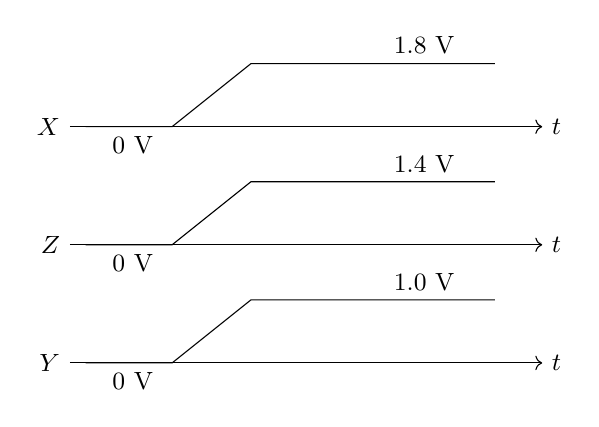
\begin{tikzpicture}[x=1cm,y=1cm,font=\small]
\foreach\y/\name/\v in {3/X/1.8,1.5/Z/1.4,0/Y/1.0}{\draw[->](0,\y)--(6,\y)node[right]{$t$};\node[left]at(0,\y){$\name$};\draw(.2,\y)--(1.3,\y)--(2.3,\y+.8)--(5.4,\y+.8);\node[above]at(4.5,\y+.8){$\v$ V};\node[below]at(.8,\y){0 V};}
\end{tikzpicture}\end{center}
\textbf{(b)} For an nMOS, assign the lower-potential terminal as source. Conducting linear operation requires $V_{DS}<V_{GS}-V_t$, equivalently $V_{GD}>V_t$; saturation requires $V_{GD}<V_t$, with equality the boundary.
The terminal directly driven by $X$ at $m1$ can reach 1.8 V. At a high charging bias, $V_{GD}=1.8-1.8=0<0.4$, so $m1$ can saturate. At lower input/discharging bias it can be linear. An ideal abrupt high step places it in saturation while charging, then cutoff at its threshold-limited endpoint; a finite ramp/other admissible bias supplies the linear interval.
For $m2$--$m6$, both data terminals are bounded by $1.8-0.4=1.4$ V. With their gates at 1.8 V, $V_{GD}\ge0.4$ V. Thus they are linear while conducting, with possible saturation-boundary or cutoff limits, and cannot enter \emph{interior} saturation under this no-body-effect/no-overshoot bound. The verifier checks 225 endpoint bias pairs in the bounded interval and explicit $m1$ examples. These are analytical admissible biases, not simulated trajectories.
\newpage
\qheading{5. Equal inverter sizes with fixed $8RC$ delay (10 points)}
The minimum nMOS has $R_n=R$, $C_{g,n}=C$. With $\mu_n=3\mu_p$ and p/n width ratio $\alpha$, $R_p=3R/\alpha$ and the next inverter's input capacitance is $(1+\alpha)C$. A transition through the first two inverters sees one rising and one falling response, so
\[T=(R_n+R_p)(1+\alpha)C=RC(1+\alpha)(1+3/\alpha).\]
The printed equality $T=8RC$ yields
\[\alpha+4+\frac3\alpha=8\quad\Longrightarrow\quad(\alpha-1)(\alpha-3)=0,
\qquad \alpha\in\{1,3\}.\]
For the same input charging activity $a_{01}$, the first two inverter output nodes each drive an equal next-stage gate load:
\[P_{sw,1+2}=2a_{01}f(1+\alpha)CV_{DD}^2.\]
Therefore $\boxed{\alpha=1}$ gives the minimum switching power subject to the required delay; its two-node gate load is $4C$, versus $8C$ for $\alpha=3$, so its modeled power is half. The final external $C_L$ is after the third inverter and is outside the bracketed first-two-stage $T$. Output diffusion/wire capacitance is not supplied and is excluded from this gate-load model.
The unconstrained fastest size would be $\alpha=\sqrt3$, giving $T=(4+2\sqrt3)RC$, but it does not satisfy the printed equality $8RC$. Matching rise/fall resistances at $\alpha=3$ is likewise not the minimum-power choice here. The student's two roots and final $\alpha=1$ agree.
\qheading{6. Static CMOS with only true literals (10 points)}
\textbf{(a) Eight MOS.} The nMOS network realizes $w(x+y+z)$ with one $w$ in series with three parallel devices. The pMOS dual is one $w$ branch in parallel with a three-device series $x,y,z$ branch. This directly gives $f=\overline{w(x+y+z)}$, needs no input complements, and uses four devices in each rail network. Each essential literal must occur in its controlling n/p network, so this conventional complementary realization attains the eight-device minimum.
\begin{center}\begin{tikzpicture}[x=0.72cm,y=0.72cm,font=\scriptsize]
\begin{scope}[thin]\mos{0.0}{0.0}{w}{0}\end{scope}
\draw(0.25,0.5)--(0.25,0.75)node[above]{$ f $};
\draw(0.25,-0.5)--(0.25,-0.75)node[below]{$ \mathrm{ANj1} $};
\node[anchor=west]at(0.55,0.0){\texttt{AN1}};
\begin{scope}[thin]\mos{4.8}{0.0}{x}{0}\end{scope}
\draw(5.05,0.5)--(5.05,0.75)node[above]{$ \mathrm{ANj1} $};
\draw(5.05,-0.5)--(5.05,-0.75)node[below]{$ V_{SS} $};
\node[anchor=west]at(5.35,0.0){\texttt{AN2}};
\begin{scope}[thin]\mos{9.6}{0.0}{y}{0}\end{scope}
\draw(9.85,0.5)--(9.85,0.75)node[above]{$ \mathrm{ANj1} $};
\draw(9.85,-0.5)--(9.85,-0.75)node[below]{$ V_{SS} $};
\node[anchor=west]at(10.15,0.0){\texttt{AN3}};
\begin{scope}[thin]\mos{14.399999999999999}{0.0}{z}{0}\end{scope}
\draw(14.649999999999999,0.5)--(14.649999999999999,0.75)node[above]{$ \mathrm{ANj1} $};
\draw(14.649999999999999,-0.5)--(14.649999999999999,-0.75)node[below]{$ V_{SS} $};
\node[anchor=west]at(14.95,0.0){\texttt{AN4}};
\begin{scope}[thin]\mos{0.0}{-2.8}{w}{1}\end{scope}
\draw(0.25,-2.3)--(0.25,-2.05)node[above]{$ f $};
\draw(0.25,-3.3)--(0.25,-3.55)node[below]{$ V_{DD} $};
\node[anchor=west]at(0.55,-2.8){\texttt{AP1}};
\begin{scope}[thin]\mos{4.8}{-2.8}{x}{1}\end{scope}
\draw(5.05,-2.3)--(5.05,-2.05)node[above]{$ f $};
\draw(5.05,-3.3)--(5.05,-3.55)node[below]{$ \mathrm{APj1} $};
\node[anchor=west]at(5.35,-2.8){\texttt{AP2}};
\begin{scope}[thin]\mos{9.6}{-2.8}{y}{1}\end{scope}
\draw(9.85,-2.3)--(9.85,-2.05)node[above]{$ \mathrm{APj1} $};
\draw(9.85,-3.3)--(9.85,-3.55)node[below]{$ \mathrm{APj2} $};
\node[anchor=west]at(10.15,-2.8){\texttt{AP3}};
\begin{scope}[thin]\mos{14.399999999999999}{-2.8}{z}{1}\end{scope}
\draw(14.649999999999999,-2.3)--(14.649999999999999,-2.05)node[above]{$ \mathrm{APj2} $};
\draw(14.649999999999999,-3.3)--(14.649999999999999,-3.55)node[below]{$ V_{DD} $};
\node[anchor=west]at(14.95,-2.8){\texttt{AP4}};
\end{tikzpicture}\end{center}
\small Eight-device complementary CMOS for Q6(a). Identically named terminals are connected. nMOS bodies use $V_{SS}$ and pMOS bodies use $V_{DD}$.\normalsize\par
\newpage
\textbf{(b) Conventional complementary CMOS: 12 MOS.}
Generate $\bar x,\bar y$ with two inverters (four MOS). The output pull-down realizes the equality function $xy+\bar x\bar y$; its pMOS dual gives the requested XOR $\bar xy+x\bar y$. The four-n/four-p complex gate plus the input inverters totals 12.
\begin{center}\begin{tikzpicture}[x=0.72cm,y=0.72cm,font=\scriptsize]
\begin{scope}[thin]\mos{0.0}{0.0}{x}{1}\end{scope}
\draw(0.25,0.5)--(0.25,0.75)node[above]{$ \bar x $};
\draw(0.25,-0.5)--(0.25,-0.75)node[below]{$ V_{DD} $};
\node[anchor=west]at(0.55,0.0){\texttt{IXP}};
\begin{scope}[thin]\mos{4.8}{0.0}{x}{0}\end{scope}
\draw(5.05,0.5)--(5.05,0.75)node[above]{$ \bar x $};
\draw(5.05,-0.5)--(5.05,-0.75)node[below]{$ V_{SS} $};
\node[anchor=west]at(5.35,0.0){\texttt{IXN}};
\begin{scope}[thin]\mos{9.6}{0.0}{y}{1}\end{scope}
\draw(9.85,0.5)--(9.85,0.75)node[above]{$ \bar y $};
\draw(9.85,-0.5)--(9.85,-0.75)node[below]{$ V_{DD} $};
\node[anchor=west]at(10.15,0.0){\texttt{IYP}};
\begin{scope}[thin]\mos{14.399999999999999}{0.0}{y}{0}\end{scope}
\draw(14.649999999999999,0.5)--(14.649999999999999,0.75)node[above]{$ \bar y $};
\draw(14.649999999999999,-0.5)--(14.649999999999999,-0.75)node[below]{$ V_{SS} $};
\node[anchor=west]at(14.95,0.0){\texttt{IYN}};
\begin{scope}[thin]\mos{0.0}{-2.8}{x}{0}\end{scope}
\draw(0.25,-2.3)--(0.25,-2.05)node[above]{$ f $};
\draw(0.25,-3.3)--(0.25,-3.55)node[below]{$ \mathrm{BNj1} $};
\node[anchor=west]at(0.55,-2.8){\texttt{BN1}};
\begin{scope}[thin]\mos{4.8}{-2.8}{y}{0}\end{scope}
\draw(5.05,-2.3)--(5.05,-2.05)node[above]{$ \mathrm{BNj1} $};
\draw(5.05,-3.3)--(5.05,-3.55)node[below]{$ V_{SS} $};
\node[anchor=west]at(5.35,-2.8){\texttt{BN2}};
\begin{scope}[thin]\mos{9.6}{-2.8}{\bar x}{0}\end{scope}
\draw(9.85,-2.3)--(9.85,-2.05)node[above]{$ f $};
\draw(9.85,-3.3)--(9.85,-3.55)node[below]{$ \mathrm{BNj2} $};
\node[anchor=west]at(10.15,-2.8){\texttt{BN3}};
\begin{scope}[thin]\mos{14.399999999999999}{-2.8}{\bar y}{0}\end{scope}
\draw(14.649999999999999,-2.3)--(14.649999999999999,-2.05)node[above]{$ \mathrm{BNj2} $};
\draw(14.649999999999999,-3.3)--(14.649999999999999,-3.55)node[below]{$ V_{SS} $};
\node[anchor=west]at(14.95,-2.8){\texttt{BN4}};
\begin{scope}[thin]\mos{0.0}{-5.6}{x}{1}\end{scope}
\draw(0.25,-5.1)--(0.25,-4.85)node[above]{$ f $};
\draw(0.25,-6.1)--(0.25,-6.35)node[below]{$ \mathrm{BPj1} $};
\node[anchor=west]at(0.55,-5.6){\texttt{BP1}};
\begin{scope}[thin]\mos{4.8}{-5.6}{y}{1}\end{scope}
\draw(5.05,-5.1)--(5.05,-4.85)node[above]{$ f $};
\draw(5.05,-6.1)--(5.05,-6.35)node[below]{$ \mathrm{BPj1} $};
\node[anchor=west]at(5.35,-5.6){\texttt{BP2}};
\begin{scope}[thin]\mos{9.6}{-5.6}{\bar x}{1}\end{scope}
\draw(9.85,-5.1)--(9.85,-4.85)node[above]{$ \mathrm{BPj1} $};
\draw(9.85,-6.1)--(9.85,-6.35)node[below]{$ V_{DD} $};
\node[anchor=west]at(10.15,-5.6){\texttt{BP3}};
\begin{scope}[thin]\mos{14.399999999999999}{-5.6}{\bar y}{1}\end{scope}
\draw(14.649999999999999,-5.1)--(14.649999999999999,-4.85)node[above]{$ \mathrm{BPj1} $};
\draw(14.649999999999999,-6.1)--(14.649999999999999,-6.35)node[below]{$ V_{DD} $};
\node[anchor=west]at(14.95,-5.6){\texttt{BP4}};
\end{tikzpicture}\end{center}
\small Complete XOR, including both generated complements; all four input cases have exactly one output rail. Identically named terminals are connected. nMOS bodies use $V_{SS}$ and pMOS bodies use $V_{DD}$.\normalsize\par
This is the minimum within a single complementary complex output gate with the required true/complement literal generators: the nonunate equality PDN needs both polarities of each input, four conducting literals, and its four-device dual. The matching student's supposed 10-MOS circuit uses $k=\overline{xy}$ and a PDN $k+xy$; since $k+xy=1$, that circuit produces constant zero and fails 01/10. Partial grading does not make it an XOR.
\textbf{If ``static CMOS'' includes transmission-gate logic, an eight-MOS XOR is available.} The paper does not explicitly state that pass gates are excluded. With the same two input inverters, use two complementary TGs as a mux: pass $y$ when $x=0$, and pass $\bar y$ when $x=1$. This is static and full swing in the ideal TG model, although it is a different design style from a single complementary PUN/PDN gate.
\begin{center}\begin{tikzpicture}[x=0.72cm,y=0.72cm,font=\scriptsize]
\begin{scope}[thin]\mos{0.0}{0.0}{x}{1}\end{scope}
\draw(0.25,0.5)--(0.25,0.75)node[above]{$ \bar x $};
\draw(0.25,-0.5)--(0.25,-0.75)node[below]{$ V_{DD} $};
\node[anchor=west]at(0.55,0.0){\texttt{IXP}};
\begin{scope}[thin]\mos{4.8}{0.0}{x}{0}\end{scope}
\draw(5.05,0.5)--(5.05,0.75)node[above]{$ \bar x $};
\draw(5.05,-0.5)--(5.05,-0.75)node[below]{$ V_{SS} $};
\node[anchor=west]at(5.35,0.0){\texttt{IXN}};
\begin{scope}[thin]\mos{9.6}{0.0}{y}{1}\end{scope}
\draw(9.85,0.5)--(9.85,0.75)node[above]{$ \bar y $};
\draw(9.85,-0.5)--(9.85,-0.75)node[below]{$ V_{DD} $};
\node[anchor=west]at(10.15,0.0){\texttt{IYP}};
\begin{scope}[thin]\mos{14.399999999999999}{0.0}{y}{0}\end{scope}
\draw(14.649999999999999,0.5)--(14.649999999999999,0.75)node[above]{$ \bar y $};
\draw(14.649999999999999,-0.5)--(14.649999999999999,-0.75)node[below]{$ V_{SS} $};
\node[anchor=west]at(14.95,0.0){\texttt{IYN}};
\begin{scope}[thin]\mos{0.0}{-2.8}{x}{1}\end{scope}
\draw(0.25,-2.3)--(0.25,-2.05)node[above]{$ f $};
\draw(0.25,-3.3)--(0.25,-3.55)node[below]{$ y $};
\node[anchor=west]at(0.55,-2.8){\texttt{TY\_P}};
\begin{scope}[thin]\mos{4.8}{-2.8}{\bar x}{0}\end{scope}
\draw(5.05,-2.3)--(5.05,-2.05)node[above]{$ f $};
\draw(5.05,-3.3)--(5.05,-3.55)node[below]{$ y $};
\node[anchor=west]at(5.35,-2.8){\texttt{TY\_N}};
\begin{scope}[thin]\mos{9.6}{-2.8}{\bar x}{1}\end{scope}
\draw(9.85,-2.3)--(9.85,-2.05)node[above]{$ f $};
\draw(9.85,-3.3)--(9.85,-3.55)node[below]{$ \bar y $};
\node[anchor=west]at(10.15,-2.8){\texttt{TYB\_P}};
\begin{scope}[thin]\mos{14.399999999999999}{-2.8}{x}{0}\end{scope}
\draw(14.649999999999999,-2.3)--(14.649999999999999,-2.05)node[above]{$ f $};
\draw(14.649999999999999,-3.3)--(14.649999999999999,-3.55)node[below]{$ \bar y $};
\node[anchor=west]at(14.95,-2.8){\texttt{TYB\_N}};
\end{tikzpicture}\end{center}
\small Eight-device static TG alternative. TY: N gate $\bar x$, P gate $x$; TYB: N gate $x$, P gate $\bar x$. Identically named terminals are connected. nMOS bodies use $V_{SS}$ and pMOS bodies use $V_{DD}$.\normalsize\par
Thus use 12 for the conventional fully complementary interpretation; if the broader static pass-logic interpretation is permitted, the displayed eight-device implementation is smaller. The alternative is kept explicit rather than silently changing the requested design style or asserting an unrestricted minimum from one topology.
\newpage
\qheading{7. Full adder (15 points)}
\textbf{(a)} The sum/carry encode the integer $x+y+c_{in}$:
\begin{center}\begin{tabular}{ccccc}\toprule$x$&$y$&$c_{in}$&$s_{out}$&$c_{out}$\\\midrule
0&0&0&0&0\\0&0&1&1&0\\0&1&0&1&0\\0&1&1&0&1\\
1&0&0&1&0\\1&0&1&0&1\\1&1&0&0&1\\1&1&1&1&1\\\bottomrule\end{tabular}\end{center}
\textbf{(b)}
\[\boxed{c_{out}=xy+xc_{in}+yc_{in}=xy+c_{in}(x+y),\qquad s_{out}=x\oplus y\oplus c_{in}.}\]
Equivalently $s_{out}=\bar x\bar yc_{in}+\bar xy\bar c_{in}+x\bar y\bar c_{in}+xyc_{in}$.
\textbf{(c) A complete 28-MOS static CMOS implementation.} Let $\bar c_{out}$ be the internal complemented carry. Generate it directly with a five-nMOS PDN for $xy+c_{in}(x+y)$ and its five-pMOS dual; an output inverter produces $c_{out}$. Use the identity
\[s_{out}=\bar c_{out}(x+y+c_{in})+xyc_{in}.\]
Its seven-nMOS PDN and seven-pMOS dual generate $\bar s_{out}$; an output inverter produces the true sum. The count is $(5+5+2)+(7+7+2)=28$. Only the three true primary inputs are needed; the required complemented carry is generated inside the circuit.
The following named-net transistor diagram includes every device, both output inverters and all intermediate series joins. It is fully complementary rather than a threshold-loss pass implementation.
\newpage
\begin{center}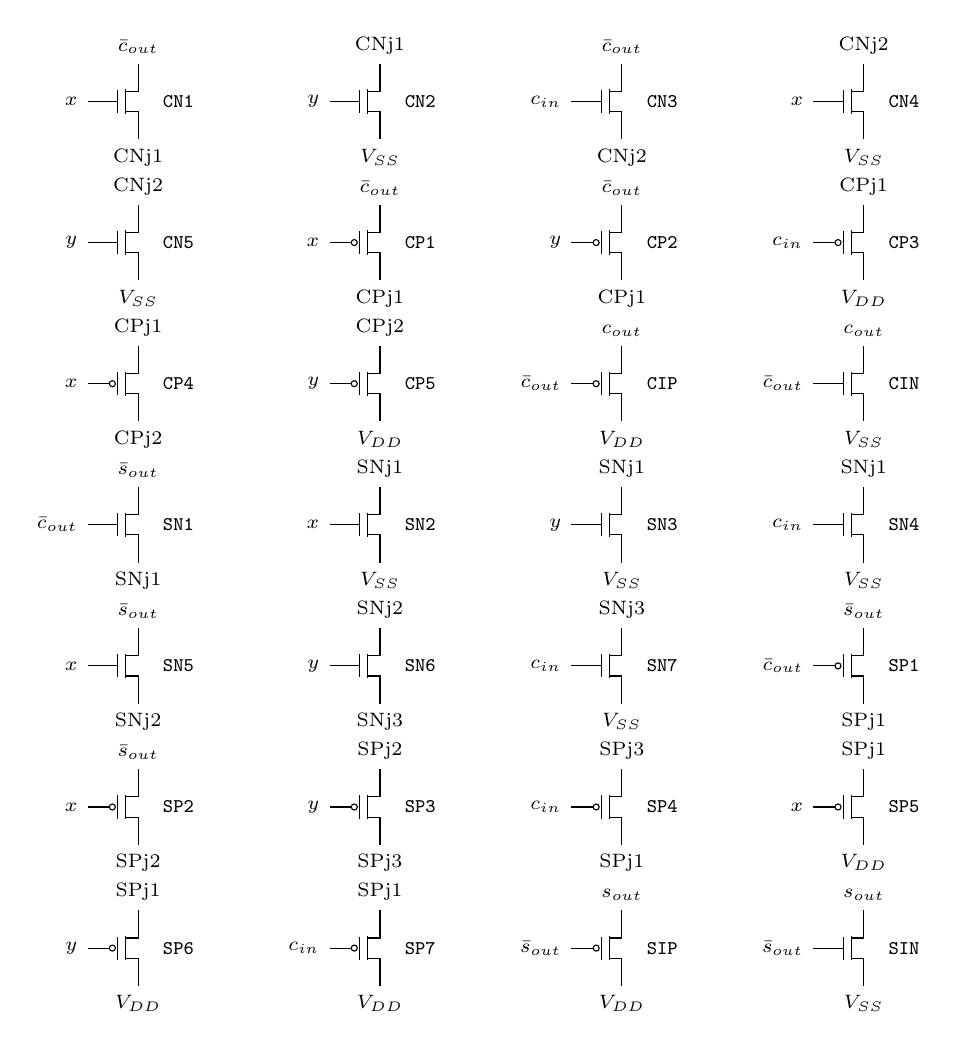
\begin{tikzpicture}[x=0.64cm,y=0.64cm,font=\scriptsize]
\begin{scope}[thin]\mos{0.0}{0.0}{x}{0}\end{scope}
\draw(0.25,0.5)--(0.25,0.75)node[above]{$ \bar c_{out} $};
\draw(0.25,-0.5)--(0.25,-0.75)node[below]{$ \mathrm{CNj1} $};
\node[anchor=west]at(0.55,0.0){\texttt{CN1}};
\begin{scope}[thin]\mos{4.8}{0.0}{y}{0}\end{scope}
\draw(5.05,0.5)--(5.05,0.75)node[above]{$ \mathrm{CNj1} $};
\draw(5.05,-0.5)--(5.05,-0.75)node[below]{$ V_{SS} $};
\node[anchor=west]at(5.35,0.0){\texttt{CN2}};
\begin{scope}[thin]\mos{9.6}{0.0}{c_{in}}{0}\end{scope}
\draw(9.85,0.5)--(9.85,0.75)node[above]{$ \bar c_{out} $};
\draw(9.85,-0.5)--(9.85,-0.75)node[below]{$ \mathrm{CNj2} $};
\node[anchor=west]at(10.15,0.0){\texttt{CN3}};
\begin{scope}[thin]\mos{14.399999999999999}{0.0}{x}{0}\end{scope}
\draw(14.649999999999999,0.5)--(14.649999999999999,0.75)node[above]{$ \mathrm{CNj2} $};
\draw(14.649999999999999,-0.5)--(14.649999999999999,-0.75)node[below]{$ V_{SS} $};
\node[anchor=west]at(14.95,0.0){\texttt{CN4}};
\begin{scope}[thin]\mos{0.0}{-2.8}{y}{0}\end{scope}
\draw(0.25,-2.3)--(0.25,-2.05)node[above]{$ \mathrm{CNj2} $};
\draw(0.25,-3.3)--(0.25,-3.55)node[below]{$ V_{SS} $};
\node[anchor=west]at(0.55,-2.8){\texttt{CN5}};
\begin{scope}[thin]\mos{4.8}{-2.8}{x}{1}\end{scope}
\draw(5.05,-2.3)--(5.05,-2.05)node[above]{$ \bar c_{out} $};
\draw(5.05,-3.3)--(5.05,-3.55)node[below]{$ \mathrm{CPj1} $};
\node[anchor=west]at(5.35,-2.8){\texttt{CP1}};
\begin{scope}[thin]\mos{9.6}{-2.8}{y}{1}\end{scope}
\draw(9.85,-2.3)--(9.85,-2.05)node[above]{$ \bar c_{out} $};
\draw(9.85,-3.3)--(9.85,-3.55)node[below]{$ \mathrm{CPj1} $};
\node[anchor=west]at(10.15,-2.8){\texttt{CP2}};
\begin{scope}[thin]\mos{14.399999999999999}{-2.8}{c_{in}}{1}\end{scope}
\draw(14.649999999999999,-2.3)--(14.649999999999999,-2.05)node[above]{$ \mathrm{CPj1} $};
\draw(14.649999999999999,-3.3)--(14.649999999999999,-3.55)node[below]{$ V_{DD} $};
\node[anchor=west]at(14.95,-2.8){\texttt{CP3}};
\begin{scope}[thin]\mos{0.0}{-5.6}{x}{1}\end{scope}
\draw(0.25,-5.1)--(0.25,-4.85)node[above]{$ \mathrm{CPj1} $};
\draw(0.25,-6.1)--(0.25,-6.35)node[below]{$ \mathrm{CPj2} $};
\node[anchor=west]at(0.55,-5.6){\texttt{CP4}};
\begin{scope}[thin]\mos{4.8}{-5.6}{y}{1}\end{scope}
\draw(5.05,-5.1)--(5.05,-4.85)node[above]{$ \mathrm{CPj2} $};
\draw(5.05,-6.1)--(5.05,-6.35)node[below]{$ V_{DD} $};
\node[anchor=west]at(5.35,-5.6){\texttt{CP5}};
\begin{scope}[thin]\mos{9.6}{-5.6}{\bar c_{out}}{1}\end{scope}
\draw(9.85,-5.1)--(9.85,-4.85)node[above]{$ c_{out} $};
\draw(9.85,-6.1)--(9.85,-6.35)node[below]{$ V_{DD} $};
\node[anchor=west]at(10.15,-5.6){\texttt{CIP}};
\begin{scope}[thin]\mos{14.399999999999999}{-5.6}{\bar c_{out}}{0}\end{scope}
\draw(14.649999999999999,-5.1)--(14.649999999999999,-4.85)node[above]{$ c_{out} $};
\draw(14.649999999999999,-6.1)--(14.649999999999999,-6.35)node[below]{$ V_{SS} $};
\node[anchor=west]at(14.95,-5.6){\texttt{CIN}};
\begin{scope}[thin]\mos{0.0}{-8.399999999999999}{\bar c_{out}}{0}\end{scope}
\draw(0.25,-7.899999999999999)--(0.25,-7.649999999999999)node[above]{$ \bar s_{out} $};
\draw(0.25,-8.899999999999999)--(0.25,-9.149999999999999)node[below]{$ \mathrm{SNj1} $};
\node[anchor=west]at(0.55,-8.399999999999999){\texttt{SN1}};
\begin{scope}[thin]\mos{4.8}{-8.399999999999999}{x}{0}\end{scope}
\draw(5.05,-7.899999999999999)--(5.05,-7.649999999999999)node[above]{$ \mathrm{SNj1} $};
\draw(5.05,-8.899999999999999)--(5.05,-9.149999999999999)node[below]{$ V_{SS} $};
\node[anchor=west]at(5.35,-8.399999999999999){\texttt{SN2}};
\begin{scope}[thin]\mos{9.6}{-8.399999999999999}{y}{0}\end{scope}
\draw(9.85,-7.899999999999999)--(9.85,-7.649999999999999)node[above]{$ \mathrm{SNj1} $};
\draw(9.85,-8.899999999999999)--(9.85,-9.149999999999999)node[below]{$ V_{SS} $};
\node[anchor=west]at(10.15,-8.399999999999999){\texttt{SN3}};
\begin{scope}[thin]\mos{14.399999999999999}{-8.399999999999999}{c_{in}}{0}\end{scope}
\draw(14.649999999999999,-7.899999999999999)--(14.649999999999999,-7.649999999999999)node[above]{$ \mathrm{SNj1} $};
\draw(14.649999999999999,-8.899999999999999)--(14.649999999999999,-9.149999999999999)node[below]{$ V_{SS} $};
\node[anchor=west]at(14.95,-8.399999999999999){\texttt{SN4}};
\begin{scope}[thin]\mos{0.0}{-11.2}{x}{0}\end{scope}
\draw(0.25,-10.7)--(0.25,-10.45)node[above]{$ \bar s_{out} $};
\draw(0.25,-11.7)--(0.25,-11.95)node[below]{$ \mathrm{SNj2} $};
\node[anchor=west]at(0.55,-11.2){\texttt{SN5}};
\begin{scope}[thin]\mos{4.8}{-11.2}{y}{0}\end{scope}
\draw(5.05,-10.7)--(5.05,-10.45)node[above]{$ \mathrm{SNj2} $};
\draw(5.05,-11.7)--(5.05,-11.95)node[below]{$ \mathrm{SNj3} $};
\node[anchor=west]at(5.35,-11.2){\texttt{SN6}};
\begin{scope}[thin]\mos{9.6}{-11.2}{c_{in}}{0}\end{scope}
\draw(9.85,-10.7)--(9.85,-10.45)node[above]{$ \mathrm{SNj3} $};
\draw(9.85,-11.7)--(9.85,-11.95)node[below]{$ V_{SS} $};
\node[anchor=west]at(10.15,-11.2){\texttt{SN7}};
\begin{scope}[thin]\mos{14.399999999999999}{-11.2}{\bar c_{out}}{1}\end{scope}
\draw(14.649999999999999,-10.7)--(14.649999999999999,-10.45)node[above]{$ \bar s_{out} $};
\draw(14.649999999999999,-11.7)--(14.649999999999999,-11.95)node[below]{$ \mathrm{SPj1} $};
\node[anchor=west]at(14.95,-11.2){\texttt{SP1}};
\begin{scope}[thin]\mos{0.0}{-14.0}{x}{1}\end{scope}
\draw(0.25,-13.5)--(0.25,-13.25)node[above]{$ \bar s_{out} $};
\draw(0.25,-14.5)--(0.25,-14.75)node[below]{$ \mathrm{SPj2} $};
\node[anchor=west]at(0.55,-14.0){\texttt{SP2}};
\begin{scope}[thin]\mos{4.8}{-14.0}{y}{1}\end{scope}
\draw(5.05,-13.5)--(5.05,-13.25)node[above]{$ \mathrm{SPj2} $};
\draw(5.05,-14.5)--(5.05,-14.75)node[below]{$ \mathrm{SPj3} $};
\node[anchor=west]at(5.35,-14.0){\texttt{SP3}};
\begin{scope}[thin]\mos{9.6}{-14.0}{c_{in}}{1}\end{scope}
\draw(9.85,-13.5)--(9.85,-13.25)node[above]{$ \mathrm{SPj3} $};
\draw(9.85,-14.5)--(9.85,-14.75)node[below]{$ \mathrm{SPj1} $};
\node[anchor=west]at(10.15,-14.0){\texttt{SP4}};
\begin{scope}[thin]\mos{14.399999999999999}{-14.0}{x}{1}\end{scope}
\draw(14.649999999999999,-13.5)--(14.649999999999999,-13.25)node[above]{$ \mathrm{SPj1} $};
\draw(14.649999999999999,-14.5)--(14.649999999999999,-14.75)node[below]{$ V_{DD} $};
\node[anchor=west]at(14.95,-14.0){\texttt{SP5}};
\begin{scope}[thin]\mos{0.0}{-16.799999999999997}{y}{1}\end{scope}
\draw(0.25,-16.299999999999997)--(0.25,-16.049999999999997)node[above]{$ \mathrm{SPj1} $};
\draw(0.25,-17.299999999999997)--(0.25,-17.549999999999997)node[below]{$ V_{DD} $};
\node[anchor=west]at(0.55,-16.799999999999997){\texttt{SP6}};
\begin{scope}[thin]\mos{4.8}{-16.799999999999997}{c_{in}}{1}\end{scope}
\draw(5.05,-16.299999999999997)--(5.05,-16.049999999999997)node[above]{$ \mathrm{SPj1} $};
\draw(5.05,-17.299999999999997)--(5.05,-17.549999999999997)node[below]{$ V_{DD} $};
\node[anchor=west]at(5.35,-16.799999999999997){\texttt{SP7}};
\begin{scope}[thin]\mos{9.6}{-16.799999999999997}{\bar s_{out}}{1}\end{scope}
\draw(9.85,-16.299999999999997)--(9.85,-16.049999999999997)node[above]{$ s_{out} $};
\draw(9.85,-17.299999999999997)--(9.85,-17.549999999999997)node[below]{$ V_{DD} $};
\node[anchor=west]at(10.15,-16.799999999999997){\texttt{SIP}};
\begin{scope}[thin]\mos{14.399999999999999}{-16.799999999999997}{\bar s_{out}}{0}\end{scope}
\draw(14.649999999999999,-16.299999999999997)--(14.649999999999999,-16.049999999999997)node[above]{$ s_{out} $};
\draw(14.649999999999999,-17.299999999999997)--(14.649999999999999,-17.549999999999997)node[below]{$ V_{SS} $};
\node[anchor=west]at(14.95,-16.799999999999997){\texttt{SIN}};
\end{tikzpicture}\end{center}
\small All 28 full-adder devices. C-prefixed complex devices generate complemented carry; S-prefixed devices generate complemented sum. Identically named terminals are connected. nMOS bodies use $V_{SS}$ and pMOS bodies use $V_{DD}$.\normalsize\par
The verifier exhausts all eight cases and checks exclusive output rails plus $s_{out}+2c_{out}=x+y+c_{in}$. The matching student's truth table and SOPs are correct. Its literal-based carry pull-down uses $\bar x\bar y+\bar x\bar c_{in}+\bar y\bar c_{in}$, which can correctly produce the true carry after output inversion, provided those complement wires exist. Its drawings omit generators for complemented primary inputs. The complete network above avoids that omission and produces both original requested true outputs with only the three true primary inputs.
\qheading{Verification and provenance}
Saved evidence includes eight majority truth rows and six complete RC networks, 64 dual-threshold logic cases, explicit passing/failing slack examples, pass-level/region examples, both feasible sizing roots, 16 Q6(a) and four Q6(b) cases with the incorrect student circuit distinguished, and eight full-adder cases. The no-body-effect bound is checked over 225 downstream endpoint pairs. Ideal rail checks do not establish analog threshold choices, transistor noise margins or process timing.
The reconstructed questions retain their printed page order, and the matching answer-photo duplicates are treated as one comparison source. No reference identity page is published. \texttt{coverage-entry.json} records all seven questions/100 points. \texttt{qa.json} records compilation and page review.
\end{document}
